\vbtitle{Equation of a Circle}

\vbdefinition{A circle can be defined as the locus of a point that moves in such a way that it maintains a constant distance from a fixed point. This fixed point is known as the center of the circle, and the constant distance is known as the radius.}

\begin{center}
    \begin{tikzpicture}
        \tzline[->](-3, -1)(4, -1){$x$}[r]
        \tzline[->](-1, -3)(-1, 3.5){$y$}[a]
        \tzcoor*(0, 0)(O){$O(x_0, y_0)$}[l]
        \tzcircle[dashed](O)(2)
        \tzcoor*(30:2)(M){$M(x, y)$}[r]
        \tzline+[->](M)(120:1)
        \tzline[dashed](O)(M){$r$}[mb]
    \end{tikzpicture}
\end{center}

\begin{align*}
    \intertext{Consider a fixed point $O(x_0, y_0)$ and a moving point $M(x, y)$ such that the distance between $O$ and $M$ is constant.}
    OM &= r \\
    \sqrt{(x - x_0)^2 + (y - y_0)^2} &= r \\
    \Aboxed{(x - x_0)^2 + (y - y_0)^2 &= r^2}\\[5mm]
\end{align*}

\begin{center}
    \begin{tikzpicture}
        \tzaxes(-3, -3)(3, 3){$x$}{$y$}
        \tzcoor*(0, 0)(O){$O$}[bl]
        \tzcircle[dashed](O)(2)
        \tzcoor*(30:2)(M){$M(x, y)$}[r]
        % \tzline+[->](M)(120:1)
        \tzline[->](O)(M){$r$}[mb]
    \end{tikzpicture}
\end{center}

\begin{align*}
    \intertext{If center of the circle is at the origin, $O(0, 0)$, then the equation of the circle becomes}
    \Aboxed{x^2 + y^2 &= r^2}\\[5mm]
\end{align*}
